\graphicspath{{chapter3/}{manuscript/}}

\chapter{\textbf{\MakeUppercase{  Intégrer les échelles individuelle et
métapopulation à travers des modèles stochastiques de population :
l'impact du climat et de la compétition sur les limites de répartition
des arbres}}}

\section{Résumé de l'article et contribution}

Bien que les modèles d'aire de répartition démographique soient utilisés
de plus en plus fréquemment pour mesurer l'effet de la dynamique
individuelle dans la définition des limites de l'aire de répartition, un
nombre croissant de preuves montrent que la performance des espèces
d'arbres n'est pas corrélée à leur répartition. Dans cette étude, nous
nous demandons si la difficulté de prédire la répartition des espèces à
partir des taux démographiques peut être expliquée par l'absence de
l'intégration de la variabilité inhérente des systèmes forestiers et
l'incertitude sous-jacente des modèles forestiers.

Pour répondre à cette question, nous avons développé un Modèle de
Projection Intégrale stochastique pour prédire la croissance
démographique intrinsèque au niveau des espèces (\(\\lambda\)) pour 31
espèces d'arbres de l'est de l'Amérique du Nord. Nous avons introduit
une nouvelle métrique pour les performances spécifiques appelée
probabilité d'habitat local approprié qui capture la stochasticité
spatio-temporelle observée dans le climat et la compétition tout en
tenant compte de l'incertitude du modèle. Notre objectif était d'étudier
l'évolution de cette probabilité dans la distribution des aires de
répartition des espèces froides à chaudes en fonction du gradient de
température annuel moyen.

Nos résultats ont révélé un déclin constant et presque linéaire de la
probabilité d'habitat local approprié à partir des frontières froides
jusqu'aux frontières chaudes et à travers les espèces. Le déplacement de
cette probabilité du centre vers les frontières froides et chaudes était
principalement influencé par le climat plutôt que par la compétition
entre les espèces. Ces résultats, étayés par une nouvelle approche
tenant compte de l'incertitude, améliorent notre compréhension de
l'interaction complexe entre le climat et la compétition définissant les
aires de répartition des espèces. Ils nous permettent également de
proposer une nouvelle théorie qui utilise la probabilité d'habitat local
approprié pour établir un lien entre les taux démographiques individuels
et la dynamique des métapopulations.

Cette étude a été conçu par Dominique Gravel et moi-même. Le modèle a
été développé par Andrew MacDonald et moi-même. Les analyses, les
figures, et la première version du manuscrit ont été réalisé par
moi-même. Dominique Gravel a contribué à la révision de ce manuscrit.

\vfill{}
\pagebreak

\begin{center}
\textbf{\MakeUppercase{Unifying individual and metapopulation scales
with stochastic population models: the effect of climate and competition
on tree range limits}} \\
Willian~Vieira, Dominique~Gravel
\end{center}

\section{Abstract}

Despite recent calls to use demographic range models to scale the effect
of individual dynamics in setting range limits, there is a growing body
of evidence showing that tree species' performance is not correlated
with their distribution. In this study, we ask whether the challenge in
predicting species distribution from demographic rates stems from
overlooking the inherent variability of forest systems and the
underlying uncertainty of forest models. We use a stochastic Integral
Projection Model to predict species-level intrinsic population growth
(\(\lambda\)) for 31 eastern North American tree species. We introduce a
novel metric for species-level performance called local suitable
probability, which captures observed spatiotemporal stochasticity in
climate and competition while accommodating model uncertainty. Our focus
is on investigating how suitable probability changes across the
cold-to-hot species range distribution over the mean annual temperature
gradient. Our findings reveal a consistent, nearly linear decline in
suitable probability from the cold to hot borders across the species.
This shift in suitable probability from the center towards the cold and
hot borders is primarily driven by climate rather than competition.
These results, supported by a novel approach accounting for uncertainty,
enhance our understanding of the nuanced interplay between climate and
competition across species ranges. We conclude by proposing a novel
theory that uses the local suitable probability to establish a link
between individual demographic rates and metapopulation dynamics.

\textbf{Keywords}: Integral Projection Models, Species
distribution, Individual variability, Environmental
stochasticity, Forest demography

\hypertarget{introduction}{%
\section{Introduction}\label{introduction}}

Climate warming poses a significant challenge for several species,
particularly for trees that struggle to follow temperature warming and
moving ranges \citep{Sittaro2017}. It is imperative to untangle the
mechanisms governing their range limits to forecast how they will
respond to climate change. The niche theory predicts that a species will
be present in suitable environmental conditions that allow the species
to have a positive growth rate \citep{Hutchinson1957}. From this theory,
we can define the geographic distribution of a species as a
manifestation of individual demographic rates, such as growth, survival,
and recruitment \citep{holt2009}. By assuming these demographic rates
change with the environment, we can predict a species' range limits
based on its individuals' performance
\citep{maguire1973niche, holt2009}.

Biotic interaction is undoubtedly an essential driver of demographic
rates and, thereby, should also range limits. A recent theoretical
framework based on the coexistence theory has been proposed to assess
how biotic interactions can scale up to affect range limits
\citep{Godsoe2017}. Formally, this framework evaluates the intrinsic
population growth rate when the focal species is rare
\citep{Chesson2000a}, both in scenarios where there is no competition
(fundamental niche) and when competitive species reach equilibrium
(realized niche). Numerous studies have explored the influence of
climate and competition on the distribution of forest trees across their
ranges. For instance, \citet{Ettinger2017} observed in field experiments
that neighboring competition constrained individual performance within
the range but facilitated better performance outside the range. Using a
dynamic forest model, \citet{Scherrer2020} showed how slow demographic
rates and negative competition reduce the uphill migration rate of 16
tree species. Despite this evidence, the application of this framework
to predict the geographic distribution of species based on demographic
rates often reveals weak correlations between the performance of tree
species and their distribution
\citep{McGill2012, Thuiller2014, Csergo2017, bohner2020, LeSquin2021, Midolo2021, Guyennon2023}.

One possible explanation for such discrepancy between demographic rates
and species distribution is the common practice of assessing performance
under average conditions and pointwise estimations, neglecting the
associated uncertainty in these estimates. In ecological models, the
uncertainty in estimation arises from three distinct sources. The first
source involves measurement errors, a factor often neglected in
ecological models \citep{Damgaard2020}. The second is process
uncertainty linked to model (mis)specification \citep{Harwood2003}. Even
with a well-defined model and precise data, models must also consider
parameter uncertainty \citep{Cressie2009, Shoemaker2020}.

Beyond data and model uncertainty, variability in demographic rates and
subsequently in the population growth rate (\(\lambda\)) arises from two
primary sources \citep{van2020}. The first is attributed to demographic
and environmental stochasticity, where individuals exposed to identical
conditions may exhibit different responses simply by chance
\citep{Caswell2009}. The second source of variability arises from
heterogeneity encountered at various scales. These differences can
manifest between individual stages that motivated the development of
structured population models \citep{Lewis1942, leslie1945}, and can
promote high species diversity in forest trees \citep{Clark2010}.
Another source of heterogeneity arises from large-scale differences in
neighboring patches, often described by the metapopulation theory
\citep{Levins1969}. This theory posits that the dynamics of occupied and
empty patches in a landscape are driven by colonization and extinction
processes. This theory posits that the dynamics of occupied and empty
patches in a landscape are driven by colonization and extinction
processes. Building on this theory, \citet{Talluto2017} used patch
variability to derive colonization and extinction rates of eastern North
American trees, revealing their distribution to be out of equilibrium
with climate. Therefore, while this result advances our understanding of
the mechanisms governing large-scale tree distributions, there remains a
need to reconcile it with local demographic dynamics, given that
colonization and extinction processes ultimately manifest from
demographic rates.

Theory predicts that the uncertainty arising from stochastic and
heterogenous processes may lead to divergent outcomes in \(\lambda\).
Demographic and environmental stochasticity may increase the uncertainty
in \(\lambda\), consequently increasing the extinction risk,
particularly for populations with low performance or low density
\citep{Holt2005, Gravel2011}. For instance, demographic stochasticity
increased the extinction risk of European forest trees at the hot edge
of their distribution \citep{Guyennon2023}. On the other hand, spatial
heterogeneity has been described as a buffering process against the
stochasticity in demographic rates, thereby increasing population
persistence \citep{milles2023}. This is particularly relevant in
nonlinear models, where Jensen's inequality predicts - for convex
response functions - that higher demographic and environmental
stochasticity increases the average population growth rate
\citep{Koons2009}. Furthermore, demographic and environmental
stochasticity influence abundance variation, indirectly impacting
\(\lambda\) through density-dependence \citep{May1978, Terry2022}. A
comprehensive understanding of the response of forest trees to climate
change requires incorporating the multiple sources of variability
arising from spatio-temporal variation and parameter uncertainty.

Here, we use a stochastic Integral Projection Model (IPM) to predict
species-level intrinsic population growth (\(\lambda\)) for 31 eastern
North American tree species. The IPM integrates the growth, survival,
and recruitment demographic rates, which vary in response to climate and
competition. By fitting each demographic rate using non-linear
hierarchical Bayesian models, we capture parameter uncertainty at both
the individual and local population scales. Additionally, our model
naturally accommodates observed spatio-temporal stochasticity in climate
and competition. Then, rather than ignoring these sources of
variability, we embrace them into \(\lambda\) by defining species
performance through a probabilistic framework. Specifically, we
introduce a novel metric called \textbf{local suitable probability},
derived from the average population growth rate and its associated
variability. This metric determines the probability of a positive
population growth rate for a species under specific climate and
competition conditions.

Our analysis is as follows. First, we used the IPM to predict
species-specific \(\lambda\) at the plot level under two conditions:
without (fundamental niche) and with (realized niche) heterospecific
competition. By replicating this calculation 100 times across all
observed plots from the same species, we can assess the variability of
\(\lambda\) arising from both spatio-temporal stochasticity in the
climate and competition and model uncertainty. As this variable
\(\lambda\) changes across space, we used these observations to model
how the species' local suitable probability changes across the mean
annual temperature. Specifically, we ask how climate and competition
affect each species' local suitable probability. Then, we investigated
how a species' local suitable probability changes from the center of its
distribution toward the cold and hot borders. Finally, we disentangle
the relative impacts of climate and competition in changing suitable
probability from the center to the borders. We conclude by discussing a
novel theory that uses the local suitable probability to establish a
link between individual demographic rates and metapopulation dynamics.

\hypertarget{methods}{%
\section{Methods}\label{methods}}

\hypertarget{population-model-demographic-components-and-uncertainty-structure}{%
\subsection{Population model, demographic components, and uncertainty
structure}\label{population-model-demographic-components-and-uncertainty-structure}}

We use an Integral Projection Model (IPM) to predict the intrinsic
population growth rate (\(\lambda\)) as a function of climate and
competition. An IPM is a powerful modeling approach that allows a full
representation of all sources of variability in demography. The IPM
serves as a mathematical formulation describing the dynamics of a
continuous trait distribution (\(z\)) within a population over discrete
time steps:

\begin{equation}
n(z', t + 1) = \int_{L}^{U} \, K(z', z, X, \theta)\, n(z, t)\, \mathrm{d}z
\label{eq:ipm}\end{equation}

In our case, the trait \(z\) is defined as the tree's diameter at breast
height (dbh), constrained between the limits \(L\) and \(U\). The
continuous distribution \(n(\cdot)\) of dbh \(z\) of a population at
time \(t\) transitions to the next time step using a projection kernel
(\(K\)). The kernel \(K\), with parameters \(\theta\) and covariates
\(X\) that are time dependent, comprises three demographic submodels:

\begin{equation}
k(z', z, \theta) = [Growth(z', z, X, \theta) \times Survival(z, X, \theta)] + Recruitment(z, X, \theta)
\label{eq:kernel}\end{equation}

The growth model assesses the probability of an individual of size \(z\)
at time \(t\) transitioning to size \(z'\) at time \(t+1\). The survival
model determines the probability of an individual with size \(z\) at
time \(t\) surviving to the next time step. Lastly, the recruitment
model determines the number of new individuals entering the population
at each time step as a function of total density \(z\). The kernel \(K\)
has the same function of the population growth rate \(r\) in a
population model, where multiplying the population distribution
\(n(z, t)\) with \(K\) gives the population distribution at the next
time step \(n(z', t+1)\). Its advantage in propagating uncertainty is
that, instead of having a matrix with fixed parameters determining the
transition rate of population individuals over time, it uses a
probability distribution with uncertainty derived from the demographic
models to project individuals over time.

With the defined \(K\), we can estimate the intrinsic population growth
rate for a determined set of conditions from the covariates \(X\) and
sampled parameters from the posterior distribution \(\theta\).
Specifically, we discretize the continuous kernel \(K\) using the
mid-point rule \citep{Ellner2016} and estimate the intrinsic population
growth rate using the dominant eigenvalue of the discretized \(K\). This
approach is a local approximation of the population growth rate at the
initial time steps.

A detailed description of the data and model development is available in
Chapter 2. In summary, we evaluated non-linear statistical models to
formulate the growth, survival, and recruitment components of the IPM,
along with their uncertainty. Each demographic sub-model varies as a
function of the mean annual temperature, mean annual precipitation, and
stand basal area of larger individuals. Each model's parameters
(\(\theta\)) are species-specific, as each model is fitted separately
for each species. Both climate variables influence each demographic
model through an unimodal link function, where each model exhibits an
optimal climate and niche breadth for temperature and precipitation.
Additionally, density dependence is integrated based on the plot's total
basal area of larger individuals. Stand density affects growth and
survival through a linear model, in which two parameters determine the
strength of interaction from conspecific and heterospecific (all species
combined) competition. For the recruitment model, the annual ingrowth
rate is modulated by conspecific stand basal area, using an unimodal
function to account for both the positive effect of seed source and the
negative effect of conspecific competition. Furthermore, the annual
survival rate of potential ingrowth individuals decreases linearly with
the stand density of heterospecific individuals. Finally, the intercept
of each growth, survival, and recruitment model incorporates plot-level
random effects to control for the variance shared within the plot-year
observations.

We use two open inventory datasets from eastern North America: the
Forest Inventory and Analysis (FIA) dataset in the United States
\citep{OConnell2007} and the permanent plots of forest inventory program
for Québec \citep{Naturelles2016}. These inventories, with multiple
individual measurements over time and space, allow us to use the
transition information between measurement years for predicting growth,
survival, and recruitment rates. We selected the 31 most abundant
species, comprising 9 conifer species and 21 hardwood species,
well-dispersed across shade tolerance and successional status
(Supplementary Material 1). These species are well distributed across
the eastern North American gradient and the sampling area covers cold
and hot range limits for most species.

\hypertarget{extracting-local-suitability-probability}{%
\subsection{Extracting local suitability
probability}\label{extracting-local-suitability-probability}}

We estimate \(\lambda\) at the local population scale, specifically at
the plot level in our study. Within a given geographic location, such as
a specific latitude where several plots are located, the variance of
\(\lambda\) among those plots arises from spatio-temporal variations in
both climate and competition covariates. For instance, climate
stochasticity introduces noise in annual temperature and precipitation,
leading to environmental variation. Similarly, even with identical
climate conditions, two locations can exhibit different community
abundance and composition, resulting in variability in the strength of
competition. Beyond these spatio-temporal environmentally-induced
variations, \(\lambda\) can still vary due to the other sources of
uncertainty discussed above.

We track demographic model uncertainty at two complementary scales:
individual and plot levels. At the individual level, plots with the same
climate and competition conditions may have different \(\lambda\) values
due to the uncertainty in the demographic sub-models. Similarly, even
with the same environmental conditions and averaged parameter values
(eliminating demographic uncertainty at the individual level), two plots
can still yield different \(\lambda\) values due to the spatial
uncertainty of each demographic model assigned among plots. Therefore,
variability in the population growth rate can arise from spatio-temporal
variations in both the environment and the parameters.

Given these different sources of variability in \(\lambda\), we define
the suitable probability as the area under the distribution for
\(\lambda \geq 1\). To estimate this, we first determine the cumulative
distribution function, \(F(x)\), from the generic probability density
function, \(\lambda = f(t)\), as follows:

\begin{equation}
F_{\lambda}(x) = P(\lambda \le x) = \int_{-\infty}^{1} f(t)dt
\label{eq:cdf}\end{equation}

This function represents the cumulative distribution from \(-\infty\) to
\(x\). Subsequently, we define the suitable probability (\(\Lambda\)) as
the complement of the cumulative distribution function for \(x = 1\):

\begin{equation}
  \Lambda = 1 - F_{\lambda}(1)
\label{eq:sp}\end{equation}

\hypertarget{modeling-suitable-probability}{%
\subsection{Modeling suitable
probability}\label{modeling-suitable-probability}}

We can evaluate the suitable probability of a species at various scales,
ranging from a single local plot up to several plots in a region. At the
plot level, sources of variability in \(\lambda\) stem from parameter
uncertainty, individual heterogeneity, and temporal variability in
climate and competition. When considering multiple plots simultaneously,
we can additionally account for spatial variability in climate and
competition, along with spatial uncertainty in plot-level parameters.

Apart from parameter uncertainty at the individual level, all other
sources of variability exhibit spatial dependence. This implies that
environmental variability (from climate, competition, or both) and
parameter uncertainty at the plot level can vary based on their spatial
location. For instance, plots at the border of the species distribution
may experience more temperature variability than those at the center.
Additionally, plot-level parameter uncertainty can be spatially
clustered, capturing potential features of demographic variability
beyond the climatic and competition covariates, such as historical
factors or local edaphic conditions.

Given that variability can be spatially dependent, we can model how
suitable probability changes across the species' range distribution,
considering both fixed climate and competition effects and the
underlying spatio-temporal variability. We are particularly interested
in how suitable probability changes from the center toward the cold and
hot ranges. For that, we categorized all species' plot-year observations
based on the gradient of mean annual temperature (MAT), divided into
cold and hot ranges using the MAT centroid among all plots for the
species (\(\frac{max(MAT) + min(MAT)}{2}\)). For instance, if a species
is observed within the 4-10°C gradient of MAT, the plots with MAT below
7°C are classified as cold, while the others are classified as hot. We
chose to use MAT instead of latitude because we are interested in the
species' climatic niche, although the two variables are highly
correlated.

We assessed suitable probability separately for the cold and hot ranges,
employing a linear model to determine the relationship between
\(\lambda\) and MAT. The spatio-temporal variability of \(\lambda\)
arising from environmental stochasticity and parameter uncertainty
influences the variance of the linear model. As this variance may change
depending on the range position, we introduce a submodel for the
variance of the linear model to be dependent on MAT. To accommodate
potential asymmetry in this variance, we use a Skew Normal Distribution
(\(SN\)) incorporating an additional parameter (\(\alpha\)) that can
introduce right or left-skewed tails to the variance:

\begin{equation}
\begin{split}
&log(\lambda) \sim SN(\xi, \omega, \alpha) \\[2pt]
&\xi = \beta_{1, \xi} \times MAT + \beta_{0, \xi} \\[2pt]
&\omega = e^{\beta_{1, \omega} \times MAT + \beta_{0, \omega}}
\end{split}
\label{eq:metamodel}\end{equation}

Here, \(\xi\) is the location parameter or the \(\lambda\) average, and
\(\omega\) is the scale representing the variance around the mean.

\hypertarget{simulations}{%
\subsubsection{Simulations}\label{simulations}}

We computed \(\lambda\) for each species based on the plot-year
observations in the dataset, considering both environmentally induced
variability and parameter uncertainty. For every observed
species-plot-year combination, we incorporated temporal stochasticity in
climate conditions by using the mean and standard deviation of mean
annual temperature and precipitation calculated from the years between
measurements. For instance, in the case of a plot observed twice, we
calculated \(\lambda\) for the second observation with climate
conditions drawn randomly from a normal distribution with mean and
standard deviation defined from climate observations within the year
interval. Similarly, temporal stochasticity in competition arises from
variation in abundance and composition between measured years. By
iteratively performing this calculation, drawing parameter values
randomly from the posterior distribution, we introduced demographic
uncertainty at the individual level. For each species-plot-year
measurement, we replicated the calculation of \(\lambda\) 100 times. By
applying this approach across all plots, we naturally incorporate
spatial variation in climate and competition conditions and spatial
uncertainty in plot-level parameters.

For each species-plot-year-replication combination, we calculated
\(\lambda\) under two simulated conditions. The first scenario excludes
competition in order to evaluate the fundamental niche, with
heterospecific competition set at zero and conspecific total population
size (N) set at 0.1. This simulation is used to assess the fundamental
niche. The second scenario is used to evaluate the invasion growth rate
with residents (the realized niche), with an evaluation of the
population growth rate when the focal species is rare (\(N=0.1\)) and
heterospecific competition is set to the observed abundance of the
competitive species. This condition simulated the population growth rate
under the realized niche.

We then fitted a linear model of \(\lambda\) for each
species-plot-year-replication as a function of the mean annual
temperature gradient. Species-specific linear models were evaluated for
the hot and cold ranges using the Hamiltonian Monte Carlo (HMC)
algorithm via the Stan software \citep[version 2.30.1][]{stan2022stan}
and the \texttt{cmdstandr} R package \citep[version 0.5.3][]{cmdstanr}.
We used a sample of 5000 plots for each species to fit the model. This
sample was necessary only for 6 out of the 31 species.

We leveraged the posterior distribution to estimate the suitable
probability of a species for any value of MAT under fundamental or
realized niches for the cold and hot ranges. Specifically, we estimated
suitable probability under four different MAT conditions encountered by
the species: at the border and the center of each cold and hot range. We
defined the border of the cold range as the minimum observed MAT for the
focal species in the dataset, while the hot range was defined as the
maximum observed MAT. The center location is defined as the centroid of
MAT for the focal species. Although the center location has the same MAT
for the cold and hot ranges, both are retained because the model is
fitted separately for the cold and hot ranges. Finally, we estimated
suitable probability for each location under no competition (fundamental
niche) and heterospecific competition (realized niche) conditions, using
the empirical cumulative distribution function over 1000 predictive
draws.

The code for the computation of each plot-year \(\lambda\) is available
at
\url{https://github.com/willvieira/forest-IPM/tree/master/simulations/lambda_plot},
and the code to model the linear model is at
\url{https://github.com/willvieira/forest-IPM/tree/master/simulations/model_lambdaPlot/}.

\hypertarget{results}{%
\section{Results}\label{results}}

\hypertarget{model-fit}{%
\subsubsection{Model fit}\label{model-fit}}

We first analyzed how the local population growth rate (\(\lambda\)) and
its variability change across the cold and hot ranges (Equation
\ref{eq:metamodel}). An example is provided at Figure
\ref{fig:res_example} with the observed distribution of \(\lambda\) and
the fit of the underlying model on the mean annual temperature gradient
for balsam fir, \emph{Abies balsamea}. Each point represents a
plot-year-replication encompassing the complete spatio-temporal sources
of variability arising from the stochastic environment and parameter
uncertainty. The black line represents the fitted model of how
\(\lambda\) changes with MAT, and the envelopes depict the 90th
quantiles of model distribution. From this uncertainty, we can deduce
the suitable probability. This example shows that the mean and variance
of \(\lambda\) decrease towards the cold border, while it does not vary
much towards the hot border. By comparing the model under heterospecific
competition with that without competition for the cold range, we
observed that while their average is similar, the uncertainty of the
model under heterospecific competition shifted downwards (Figure
\ref{fig:res_example}, bottom left).

\hypertarget{fig:res_example}{%
\begin{figure}
\centering
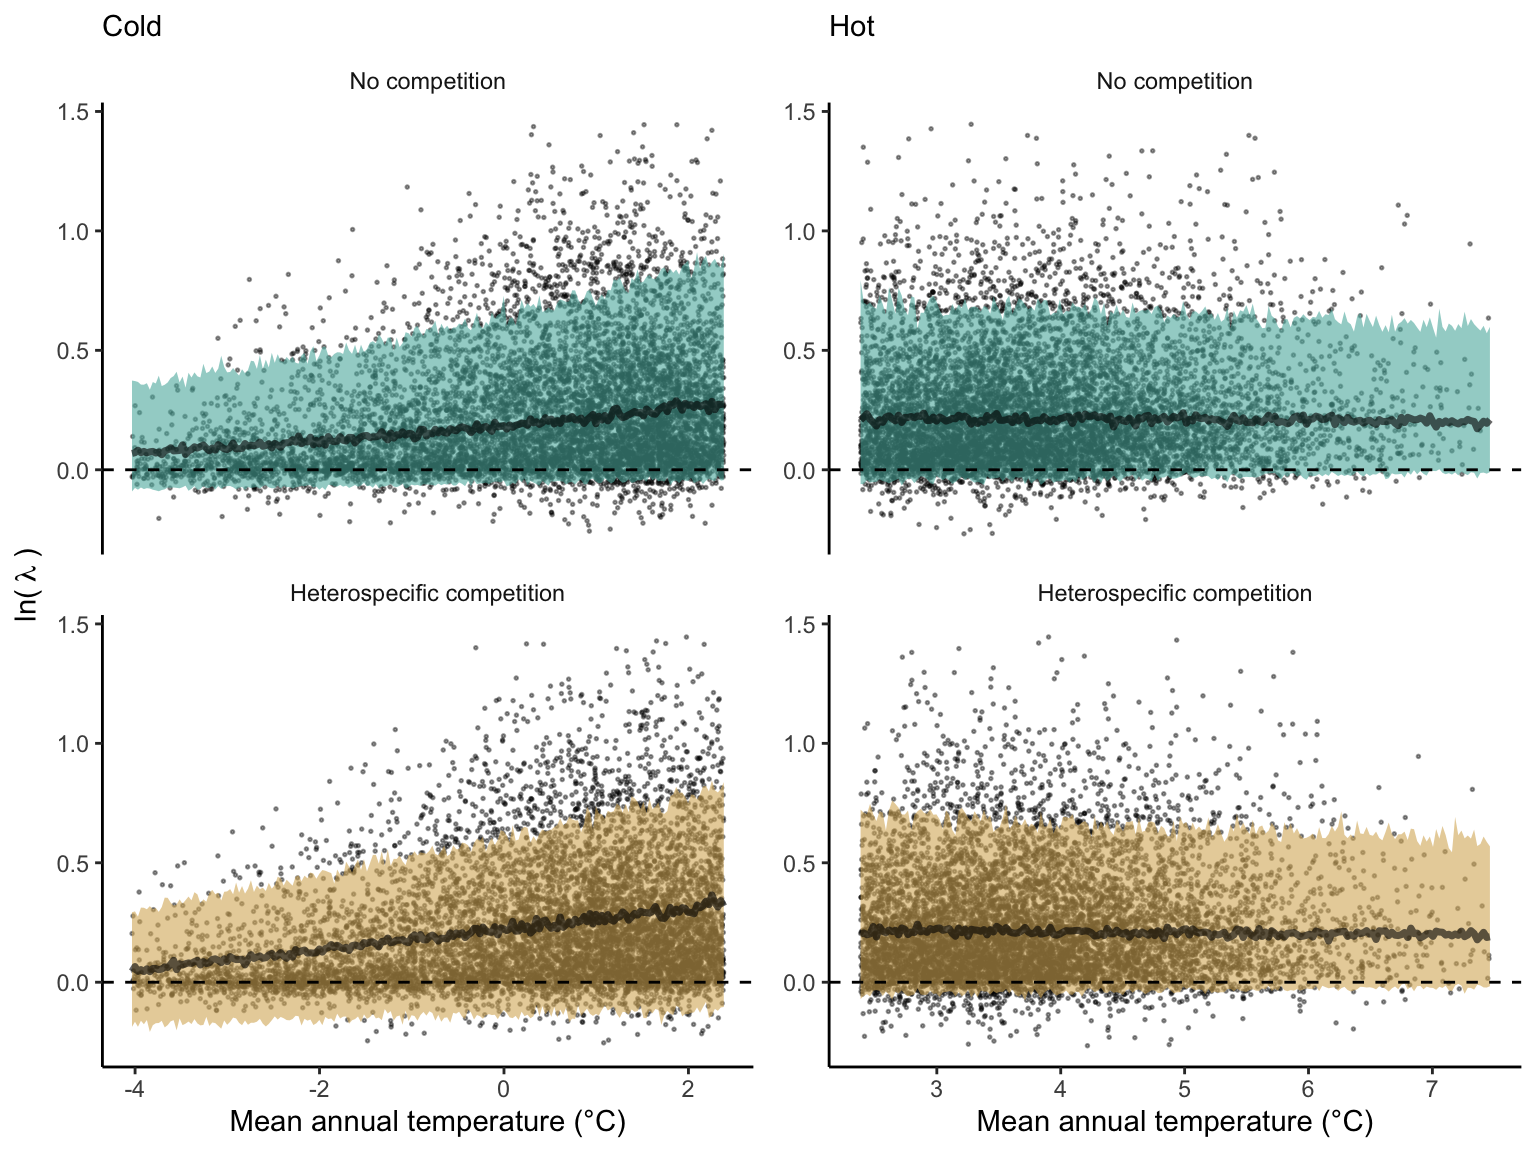
\includegraphics[width=1\textwidth,height=\textheight]{manuscript/figs/fig-res_example-1.png}
\caption[{Distribution of stochastic population growth rate
(\(\lambda\)) for \emph{Abies balsamea} over the mean annual temperature
gradient for different conditions.}]{Distribution of stochastic
population growth rate (\(\lambda\)) for \emph{Abies balsamea} over the
mean annual temperature gradient for cold (left panels) and hot (right
panels) ranges under no competition (fundamental niche) and
heterospecific competition (realized niche). The dots represent
\(\lambda\) over the plot-year-replication combinations. The model's
average line and 90\% prediction intervals are estimated using 500 draws
from the posterior distribution.}
\label{fig:res_example}
\end{figure}
}

We then investigated the local suitability probability using the
empirical cumulative distribution approach (Equation \ref{eq:sp}) from
the linear model predictions. The Figure \ref{fig:sp-example} shows the
suitable probability expected over the mean annual temperature of the
same species. We observed that the local suitability probability was
reduced towards the cold border, with a stronger reduction under
heterospecific competition (yellow curve). We can also observe that the
decrease in suitable probability towards the border is nonlinear,
becoming more substantial for heterospecific competition than for the
no-competition condition.

The model fit and the estimation of suitable probability across the
temperature gradient for all species are presented in Supplementary
Material 2. We observed for most species a decrease of the climate
effect at one border while the other remained unchanged. Additionally, a
few species displayed a clear linear pattern of decreasing suitable
probability from the cold to the hot border, with only one species
(\emph{Betula papyrifera}) having a decrease at both borders.
Conversely, under the competition effect, most species exhibited a
decrease in suitable probability at the hot border and an increase at
the cold border, indicating a linear rise in the impact of competition
from the cold to the hot border of the distribution.

\hypertarget{fig:sp-example}{%
\begin{figure}
\centering
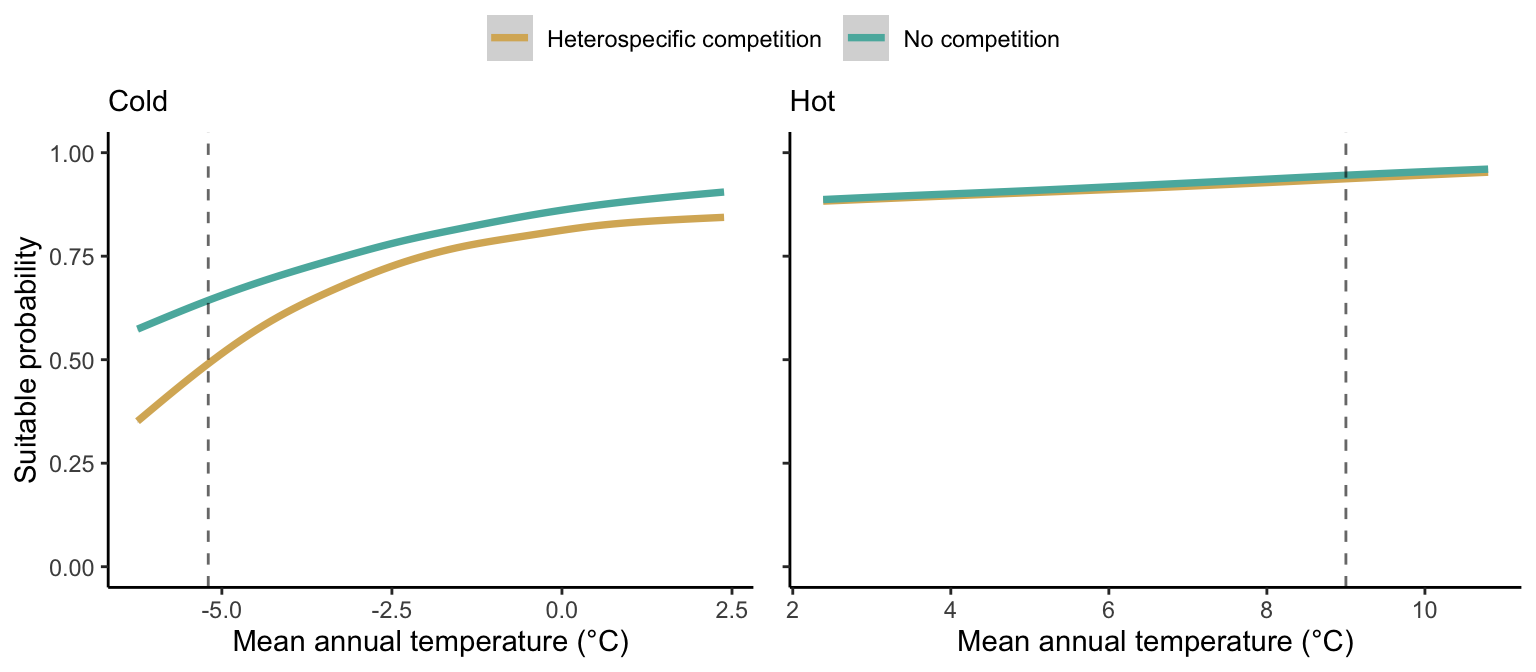
\includegraphics[width=1\textwidth,height=\textheight]{manuscript/figs/fig-sp-example-1.png}
\caption[{Suitable probability of \emph{Abies balsamea} over the mean
annual temperature gradient for cold and hot ranges under no competition
(green) and heterospecific (yellow).}]{Suitable probability of
\emph{Abies balsamea} over the mean annual temperature gradient for cold
and hot ranges under no competition (green) and heterospecific (yellow).
The vertical dotted line represents the range limits of the MAT observed
in the dataset.}
\label{fig:sp-example}
\end{figure}
}

\hypertarget{effect-of-climate-and-competition-on-suitable-probability-for-the-center-and-border-distributions}{%
\subsubsection{Effect of climate and competition on suitable probability
for the center and border
distributions}\label{effect-of-climate-and-competition-on-suitable-probability-for-the-center-and-border-distributions}}

We investigated the effect of climate and competition on the suitable
probability at the border and center of the temperature range
distribution for all species. Because the border and center positions
are relative to each species, we could not represent the continuous
trend in suitable probability across the MAT for all 31 species
together. Instead, we extracted the local suitable probability with and
without heterospecific competition for four locations across the MAT
gradient (Figure \ref{fig:sp_comp_vs_nocomp2}). Overall, suitable
probability was high among the species, with an average of 0.78. Among
the four locations, species presented a lower suitable probability at
the border of the hot range, with an average of 0.67. Across the
temperature range, there is a monotonic decrease in suitable probability
from the cold border toward the hot border.

\hypertarget{fig:sp_comp_vs_nocomp2}{%
\begin{figure}
\centering
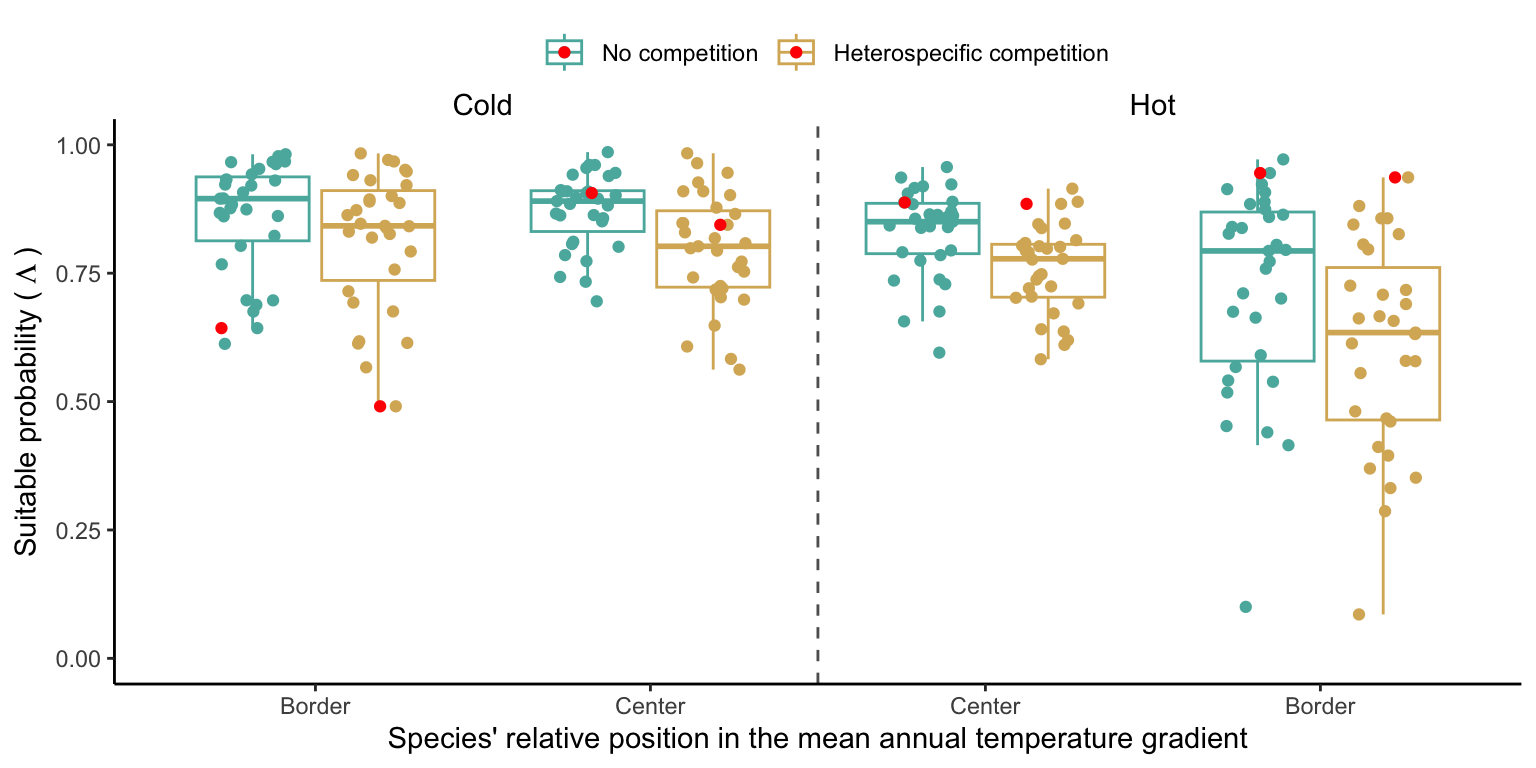
\includegraphics[width=1\textwidth,height=\textheight]{manuscript/figs/fig-sp_comp_vs_nocomp2-1.png}
\caption[{Estimated suitable probability for the 31 forest species
across across the center and border of the cold and hot
ranges.}]{Estimated suitable probability for the 31 forest species
across across the center and border of the cold and hot ranges. The
x-axis represents the mean annual temperature gradient similar to Figure
\ref{fig:sp-example}, but is discretized at the border and center limits
relative to each species. We highlighted the balsam fir species in red.
Note that we omitted the parameter uncertainty of each species in this
figure to avoid overlap and increase clarity.}
\label{fig:sp_comp_vs_nocomp2}
\end{figure}
}

We further disentangle the influence of competition from that of climate
by calculating the difference between suitable probability under
heterospecific competition and without competition. A negative
difference signifies competition reduces suitable probability, while
positive differences indicate an increase. Across the four climate
locations, heterospecific competition consistently reduced suitable
probability for most species, with the magnitude of reduction
intensifying from the cold to the hot border (Figure S1). This suggests
that the decline in suitable probability observed from the cold to the
hot border (Figure \ref{fig:sp_comp_vs_nocomp2}) results from the
combined effect of climate and competition.

\hypertarget{suitable-probability-change-from-center-to-border}{%
\subsubsection{Suitable probability change from center to
border}\label{suitable-probability-change-from-center-to-border}}

We investigated the relative effect of climate and competition on
changing suitable probability from the center to the border of the
species distribution (Figure \ref{fig:diff_sp_hist}). A positive
relative difference indicates an increase in suitable probability from
the center towards the border, while a negative difference indicates a
decrease. Most species exhibited a decrease in suitable probability at
the hot border relative to the center. Alternatively, most species
showed a reduction in the effect of competition toward the cold border.
However, the climate effect in the cold range was more variable, with
some species experiencing an increase and others a decrease in suitable
probability. Overall, the relative difference in suitable probability
from the center toward the cold and hot borders was more influenced by
climate rather than competition.

\hypertarget{fig:diff_sp_hist}{%
\begin{figure}
\centering
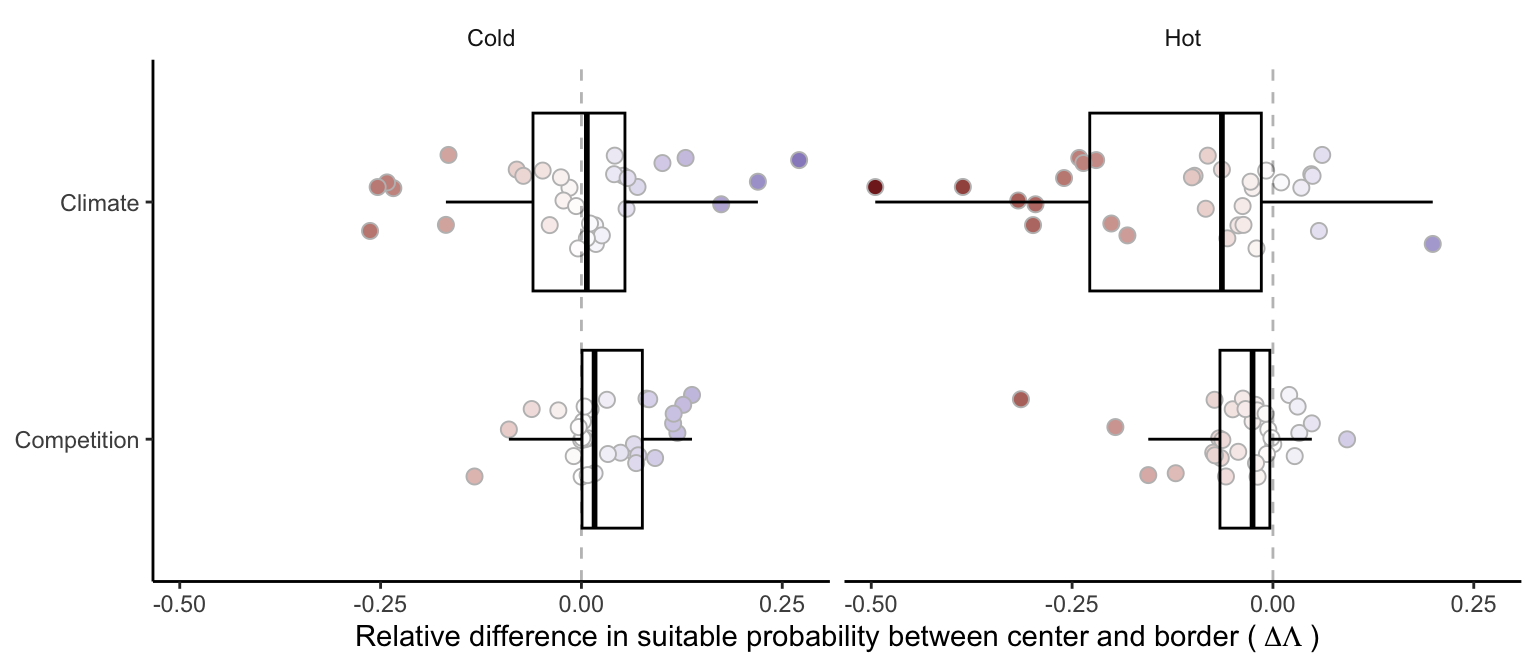
\includegraphics[width=1\textwidth,height=\textheight]{manuscript/figs/fig-diff_sp_hist-1.png}
\caption[{Difference in suitable probability for climate and competition
effects over the cold and hot ranges.}]{Difference in suitable
probability for climate and competition effects over the cold and hot
ranges. Negative values denote a decrease in species suitable
probability from the center towards the distribution border, while
positive values indicate an increase. Specifically, a negative value for
climate at the hot (or cold) range signifies a reduction in suitable
probability as temperature rises (or falls) towards the border. Boxplots
determine the 25-75 quantile distribution among the species.}
\label{fig:diff_sp_hist}
\end{figure}
}

\hypertarget{discussion}{%
\section{Discussion}\label{discussion}}

Understanding the mechanisms shaping species distribution is imperative
to face ongoing global changes. We acknowledged and integrated various
sources of variability in the population growth rate of forest trees,
contributing to an improved understanding of forest dynamics in an
uncertain world. Introducing a novel metric, we quantified the relative
impacts of climate and competition on the change in suitable probability
across species distributions. Our findings revealed a nearly linear
reduction in suitable probability from the cold to hot borders. Notably,
the predominant influence on the relative difference in suitable
probability from the center toward the border was attributed to climate
rather than competition. These results, supported by a novel approach
accounting for uncertainty, enhance our understanding of the nuanced
interplay between climate and competition across species ranges.

The suitable probability was high across all species and range
locations, with only around 5\% of all species-location combinations
having a suitable probability below the 0.5 threshold. This is primarily
attributed to most species exhibiting a high positive population growth
rate across their current range distribution. Additionally, the
spatio-temporal variability in the environment and the parameter
uncertainty in the plot may contribute to the elevated average
population growth rate due to nonlinear averaging. This aligns with
theoretical \citep{Schreiber2009} and empirical \citep{Crone2016}
studies suggesting that spatial heterogeneity should increase the
population growth rate.

Competition significantly reduces local suitability across all range
locations, with a stronger and more consistent effect at the cold
border, contributing to the ongoing debate surrounding its significance
in setting range limits. Despite several studies emphasizing the effect
of competition compared to climate on the demographic rates of forest
trees \citep{Zhang2015, Kaber2021, LeSquin2021}, debates persist
regarding whether this effect at the local scale translates to the
biogeographic distribution of species
\citep{Soberon2007, CopenhaverParry2017}. Our findings support the
\citet{Godsoe2017} hypothesis and a growing body of evidence
\citep{Scherrer2020, Shi2020, Paquette2021, Lyu2022} showing that the
effect of competition on the intrinsic population growth rate can indeed
contribute to range limits.

The decline in suitable probability from the cold to the hot border
suggests a predominantly linear, rather than unimodal, relationship with
temperature for most species. This result is consistent with reduced
population growth rates in North American
\citep{schultz2022, LeSquin2021} and European \citep{Guyennon2023}
forest trees, except for the contrasting pattern observation by
\citet{Purves2009}. The higher suitable probability in the cold range
compared to the hot range could be attributed to multiple factors.
First, species may still follow their climate niche post the last
glaciation, explaining why the current cold range limit does not align
with the expected niche distribution \citep{Svenning2007}, potentially
leading to a colonization debt \citep{Talluto2017}. Notably, four of the
six species exhibiting a significant decrease in suitable probability
from the center toward the cold range were already at the extreme cold
observed in the dataset (Figure S4).

Our model may however overlook crucial drivers of species performance,
despite capturing a substantial amount of variation from parameter
uncertainty at the plot level. Factors such as the impact of extreme
temperature and precipitation on phenology can influence tree range
limits \citep{Morin2007}. Beyond covariates and plot-level uncertainty,
incorporating temporal uncertainty at the plot level, accounting for
spatio-temporal covariance, could likely capture additional sources of
variation in demographic rates. While our approach considers temporal
stochasticity in climate and competition, which affect species range
size \citep{Holt2022}, there remains temporal variation in demographic
rates beyond these covariates. This variability, possibly captured with
random effects at the plot level, can influence range limits based on
the degree of temporal autocorrelation and its relationship with the
range \citep{Benning2022}. For instance, an empirical study on perennial
herbaceous species demonstrated that temporal environmental
stochasticity reduced the population growth rate relative to the average
\citep{Crone2016}. In our study, this temporal variability is
particularly relevant for survival (due to disturbance) and recruitment
(due to phenology) rates because, in addition to having high temporal
variability \citep{Clark1999a, Leite2023}, they represent the most
significant drivers of population growth rate (Chapter 2).

The effect of competition, similar to climate, increased from the center
towards the border of the hot range, contrary to \citet{Kunstler2021},
who found no difference in the competition effect between the center and
border of the species. Additionally, our results deviate from the
Species Interactions-Abiotic Stress Hypothesis, predicting a stronger
competition effect in less stressful climate conditions
\citep{Louthan2015}. When considering the relative position of the
species across the temperature gradient, only the effect of climate at
the cold range changed with temperature. This indicates that most
species have a similar or higher suitable probability at the border of
the cold range compared to their center distribution. We further tested
whether the species' range size affects the relative difference in
suitable probability; while the absolute values change, the pattern
among the species remains unchanged.

The climate gradient of temperature had a more significant effect than
competition in changing the suitable probability of forest trees. This
means that mean annual temperature, along with all latent variables,
better explains how suitable probability changes across the temperature
range. The choice of using only mean annual temperature as an
explanatory variable for the variance of \(\lambda\) can be improved.
For instance, the model could be built accounting for mean annual
temperature and precipitation to predict the complete two-dimensional
distribution of the species' climate niche. Plot random effects could be
further used to account for the nestedness of the data design, allowing
the proper separation of the total variance of the metamodel into
variance arising from individual- and plot-level demographic
uncertainty. While we have assumed climate variability as independent
and identically distributed random variables, this assumption can be
relaxed to include temporal autocorrelation. Autocorrelated
environmental fluctuation can significantly change a species' range
limits due to nonlinear averaging \citep{Benning2022, Holt2022}. Lastly,
although coexistence theory assumes the abundance of competitors to be
at equilibrium \citep{Chesson2000a}, testing this assumption remains
practically impossible.

Despite the many ways of improving our study, there is a growing body of
evidence indicating a mismatch between performance and occurrence
\citep{McGill2012, Thuiller2014, Csergo2017, bohner2020, LeSquin2021, Midolo2021, Guyennon2023}.
Our approach can better capture the nuanced effect of climate and
competition along with the spatio-temporal variation in \(\lambda\), yet
it was not enough to fully predict tree range limits. Since species
distribution is influenced by processes at multiple scales
\citep{McGill2010, Heffernan2014}, it is challenging to rely on a single
individual-level performance metric to predict it all \citep{Evans2016}.
For instance, dispersion plays a crucial role in changing species
distribution at larger spatial scales, either reducing its extent due to
limited dispersal or increasing it through source-sink dynamics
\citep{Pulliam2000}. We propose that our novel metric, local suitable
probability, can be a key unifying factor linking local and landscape
scales.

Forest trees exhibit variation in their frequency of occurrence across
distribution gradients, yet their relative abundance remains consistent
when present \citep{Canham2010}. Such observation implies that assessing
forest distribution should focus on colonization and extinction patch
dynamics rather than local performance \citep{Canham2017}. However,
instead of restricting models to either local or large scales, we
propose using the local suitable probability to reconcile the local
demographic dynamics with the metapopulation theory. Colonization and
extinction processes, as described by metapopulation theory
\citep{Levins1969}, are well-suited for describing the mosaic of forest
successional stages at the landscape scale resulting from natural
disturbances and succession. However, an implicit assumption is that
unoccupied patches are necessarily available for colonization. We relax
this assumption and quantify patch availability using the local suitable
probability metric (\(\Lambda\)). Take an ensable of patches (\(p\))
where individuals can arrive and establish empty patches through
colonization (\(\alpha\)), and occupied patches can become empty through
extinction (\(\varepsilon\)): Considering an ensemble of patches (\(p\))
where individuals can arrive and establish in empty patches through
colonization (\(\alpha\)), and occupied patches can become empty through
extinction (\(\varepsilon\)), the integrated metapopulation model
becomes:

\[
\frac{dp}{dt} = \alpha p (\Lambda - p) - \varepsilon p
\]

With this formulation, rather than having \(1 - p\) available patches
for colonization, we have \(\Lambda - p\). Therefore, when \(\lambda\)
and its variability are high, the local suitable probability equals 1,
indicating that all non-occupied patches are available. Conversely, as
the local suitable probability decreases, the proportion of non-occupied
patches available for colonization is reduced. This integrative approach
allows one to account for both the local (e.g.~competition and climate)
and landscape (e.g.~fire disturbances and dispersal) drivers of forest
dynamics when assessing tree distribution.

\newpage

\singlespacing
{\renewcommand{\bibname}{References}
\renewcommand{\bibsection}{\section{\bibname}}
\bibliography{chapter3/manuscript/references}}
\bibliographystyle{styles/myBEAS}
